\documentclass[10pt,a4paper]{article}
\usepackage[utf8]{inputenc}
\usepackage[T1]{fontenc}

\usepackage{graphicx}

\usepackage[]{exercise}


\title{Electromagnetic Fields Exercises\\ \vspace{0.5cm} \large{(under heavy construction)}}
\author{Bartosz Sawicki \\ \small{Faculty of Electrical Engineering, Warsaw University of Technology}}

\begin{document}

\maketitle

\noindent\textbf{From authors:}\\
This set of exercises is going to rapidly grow during this semester. Please follow changes. 

Tekst napisany jest po angielsku ze względu na studentów kierunku "Electrical Engineering". Jednak polskojęzyczni studenci nie powinni mieć problemów ze zrozumieniem ich prostego języka.

Difficulty of the exercises are indicated by the number of asterisks. 

source file: \verb+https://github.com/sawickib/emfe+

\vspace{0.3cm}
\begin{flushright}
Bartosz.Sawicki@ee.pw.edu.pl
\end{flushright}

\tableofcontents

\section{Vector algebra and differential operators}

\begin{Exercise}[difficulty=1]
There are given vectors $\vec A = 2 \vec{i} - 4\vec{k}$, $\vec B = [5, 0, 1]$ and scalar $c = 8$. Determine results of:

\begin{itemize}
\item $\vec A + (c \vec B)$
\item $\vec A \cdot \vec A - \vec B \times \vec B$
\item $(\vec B - \vec A) \cdot \vec A$
\end{itemize}

\end{Exercise}


\begin{Exercise}[difficulty=1]
Find an angle between vectors $[1,0,0]$ and $[1,2,0]$. Determine dot product and cross product of them.
\end{Exercise}


\begin{Exercise}[difficulty=1]
Show that $\vec{i}\times\vec{j} = \vec{k}$.
\end{Exercise}


\begin{Exercise}[difficulty=2]
Having vector fields $\vec A (x,y,x) = [3z^2, x, 0]$ and $\vec B (x,y,z) = y\vec{i} + x\vec{j}$, find solution of $\nabla \cdot (\vec A \times \vec{B})$
\end{Exercise}

\begin{Exercise}[difficulty=2]
Consider two vector fields defined as $\vec{A} = 2y\vec{i}+4\vec{j}+6z\vec{k}$, $\vec{B} = [ x^2, -x^2, 0]$. Find:
\begin{itemize}
\item $ \nabla \cdot \vec{B} $
\item $ {curl}( \vec A )$
\item $ \nabla ( \vec A + \vec B )$
\end{itemize}
\end{Exercise}

\begin{Exercise}[difficulty=2]
Using operator definitions prove identities:
\begin{itemize}
\item $ \nabla \cdot (\nabla \times \vec{A}) = 0$
\item $ \nabla \times \nabla = 0 )$
\item $ \vec{A} \times \vec{B} = - \vec{B} \times \vec{A} $
\end{itemize}
\end{Exercise}

\section{Electrostatics}


\begin{Exercise}[difficulty=1]
Using Gauss law find a electric field $E$ in vicinity of point charge $Q$.
\end{Exercise}

\begin{Exercise}[difficulty=2]
Show that Coulomb's law can be derived from Gauss law.
\end{Exercise}

\begin{Exercise}[difficulty=2,label=e2]
Find electric field $\vec{E}$ in point $P$, which is exactly in the middle between two point charges $Q_1$ and $Q_2$. 
%\begin{center}
%\includegraphics[scale=0.1]{test.pdf} 
%\end{center}
\end{Exercise}

\section{Current field}

\begin{Exercise}[difficulty=1]
Calculate current density in the wire (circular with diameter 1mm) if total current is 10 A.
\end{Exercise}

\begin{Exercise}[difficulty=1]
Find resistance of cable ....
\end{Exercise}

\section{Magnetic field}

\begin{Exercise}[difficulty=1]
Find direction and value of magnetic field H produced by current I in the point P. 
\begin{center}
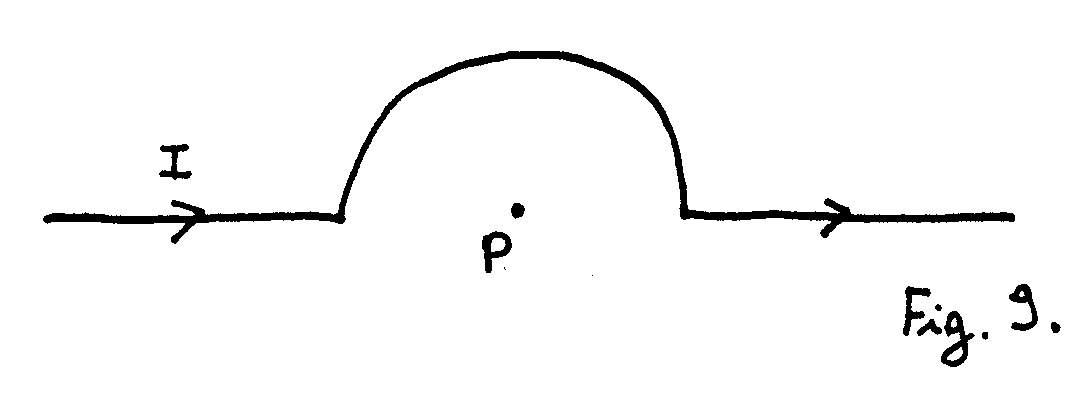
\includegraphics[width=0.4\textwidth]{img/fig_m1.png} 
\end{center}
\end{Exercise}

\begin{Exercise}[difficulty=3]
Using Ampere's Circular Law describe distribution of magnetic field vector inside, and outside coaxial cable.
\begin{center}
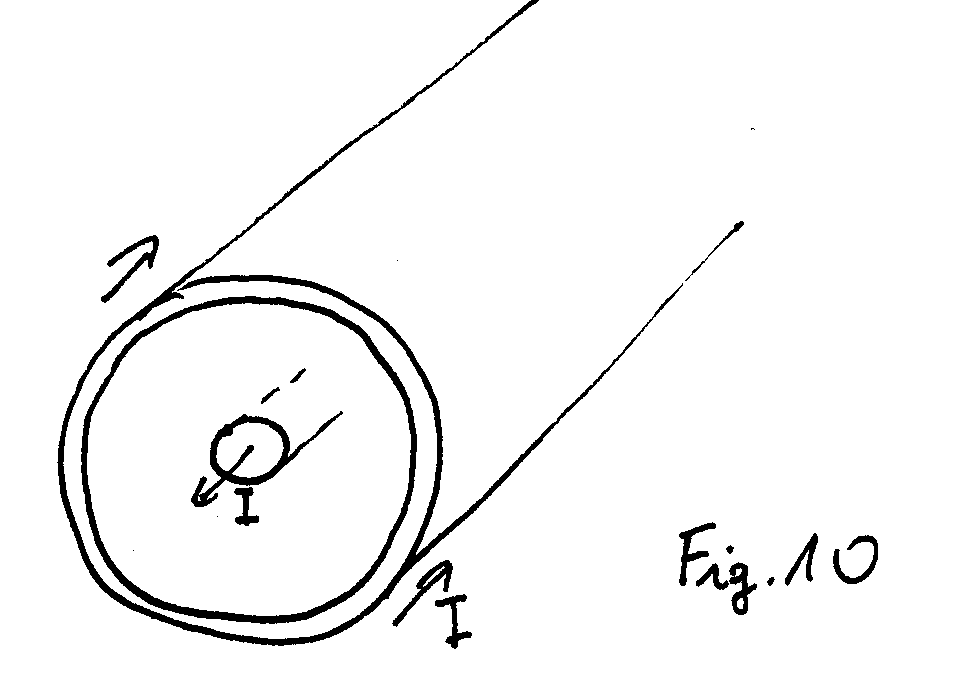
\includegraphics[width=0.4\textwidth]{img/fig_m2.png} 
\end{center}
\end{Exercise}

\begin{Exercise}[difficulty=2]
Two long, parallel cables with the same values but opposite directions of DC current are producing magnetic field around them. Find H distribution on the plane defined by two cables. 
\begin{center}
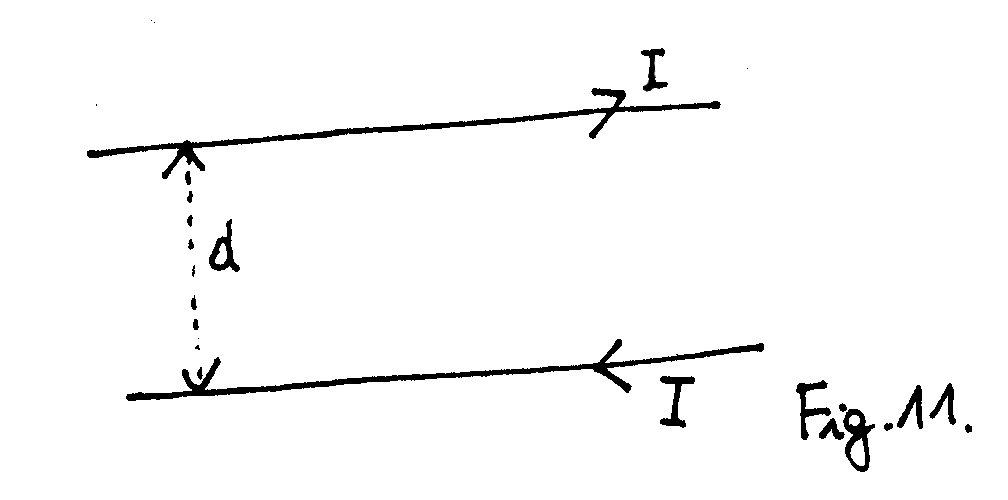
\includegraphics[width=0.4\textwidth]{img/fig_m3.png} 
\end{center}
\end{Exercise}



\end{document}